%!TEX root = paper.tex

\begin{figure}
	\begin{subfigure}{\linewidth}
		\centering
		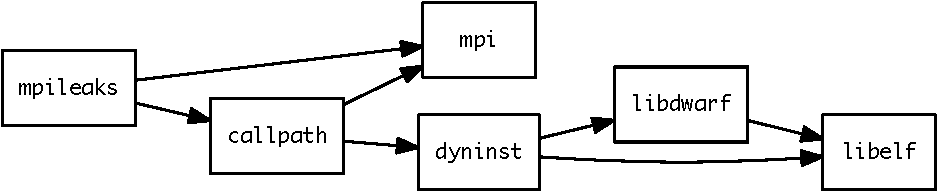
\includegraphics[width=\columnwidth]{specs/mpileaks.pdf}
		\caption{
			Spec for {\tt mpileaks}
			\label{fig:specs-mpileaks}
		}
	\end{subfigure}
%
	\begin{subfigure}{\linewidth}
		\centering
		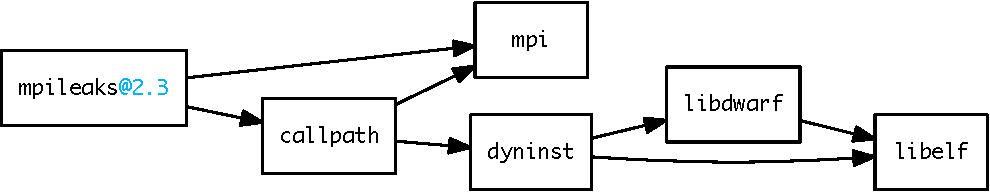
\includegraphics[width=\columnwidth]{specs/mpileaks-version}
		\caption{
			{\tt mpileaks@2.3}
			\label{fig:specs-mpileaks-version}
		}
	\end{subfigure}
%
	\begin{subfigure}{\linewidth}
		\centering
		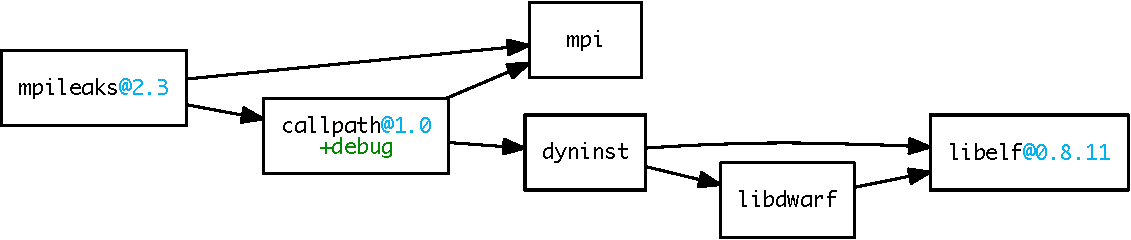
\includegraphics[width=\columnwidth]{specs/mpileaks-abstract.pdf}
		\caption{
			{\tt mpileaks@2.3 \^{}callpath@1.0+debug \^{}libelf@0.8.11}
			\label{fig:specs-mpileaks-abstract}
		}
	\end{subfigure}
%
	\caption{
		Constraints applied to {\tt mpileaks} specs.
	}
\end{figure}



\subsection{Spack Specs}\label{sec:specs}

Using the simple script in Figure~\ref{fig:mpileaks}, Spack can build many different
versions and configurations of the {\tt mpileaks} package.  In traditional port systems, 
package code is structured to build a single version of a package, but in Spack, each
package file is a {\it template} that can be built in many different ways.  The build is
{\it parameterized} so that it can be configured many different ways.  
Spack calls a single build configuration a {\it spec},
 and the {\tt spec} object passed to {\tt install()} 
is how the Spack system encapsulates build parameters for package authors.

\subsubsection{Structure}
To understand how specs work, consider the {\tt mpileaks} package structure.  
Metadata in the {\tt Mpileaks} class ({\tt version}, {\tt depends\_on}, etc.) describe
its relationships with other packages.  There are two direct dependencies: 
the {\tt callpath} library and {\tt mpi}.  Spack recursively inspects the class definitions
for each dependency and constructs a graph of their relationships.  The result
is a directed, acyclic graph (DAG) of dependencies\footnote{Spack currently disallows
circular dependencies.}.  
%
To guarantee a consistent build, and to avoid ABI incompatibility, the DAG
is constructed so that there is only {\it one} version of any particular package.  Note
the distinction: while Spack can install arbitrarily many configurations of any package,
no two configurations of the same package will ever appear in the same build DAG.

DAGs for {\tt mpileaks} are shown in Figure~\ref{fig:specs}.
Each node is a package and has five configuration parameters that control
how it will be built: 1) the package version, 2) the compiler to
build with, 3) the compiler version, 4) named compile-time build options, or {\it variants},
and 5) the target architecture.  


\subsubsection{Configuration Complexity}
A spec DAG has many degrees of freedom, and it is not reasonable to expect users to
understand or specify all of them.  In our experience at LLNL, the typical user
only cares about a small number of build constraints (if any), and does not know enough to
specify the rest. For example, a user may know that a certain version of a library like
{\tt boost} is required, but only cares that other build parameters are set so that
the build will succeed.
%
Configuration complexity makes the HPC software ecosystem difficult to manage: there are
simply too many parameters. However, the small set of important build constraints can be
very specific, so we have two competing concerns.  We need the ability to specify details
of the configuration space, without the complexity of remembering all of them.

\subsubsection{Spec Syntax}\label{sec:syntax}

\begin{figure}
\begin{grammar}
  <spec>         ::= <id> [ constraints ]

  <constraints>   ::= \{ `@' <version-list> | `+' <variant> \newline
                   | `-' <variant> ~~~| `~' <variant> \newline
                   | `\%' <compiler> ~| `=' <architecture> \} \newline
                  [ <dep-list> ]

  <dep-list>  ::= \{ `\textsf \textasciicircum' <spec> \}

  <version-list> ::= <version> [ \{ `,' <version> \} ]

  <version>      ::= <id> | <id> `:' | `:' <id> | <id> `:' <id>

  <compiler>     ::= <id> [ <version-list> ]

  <variant>      ::= <id>

  <architecture> ::= <id>

  <id>           ::= [A-Za-z0-9_][A-Za-z0-9_.-]*
\end{grammar}
\caption{
	EBNF grammar for spec expressions.
	\label{fig:grammar}
}
\end{figure}


\begin{table*}\centering
\begin{tabular}{|r|p{2.4in}|p{4in}|}
\hline
& {\bf Spec} & {\bf Meaning} \\
\hline
\hline
1&\small\verb|mpileaks|                         & \small {\tt mpileaks} package, no constraints. \\\hline
2&\small\verb|mpileaks@1.1.2|                   & \small {\tt mpileaks} package, version 1.1.2. \\\hline
3&\small\verb|mpileaks@1.1.2 %gcc|              & \small {\tt mpileaks} package, version 1.1.2, built with {\tt gcc} at the default version. \\\hline
4&\small\verb|mpileaks@1.1.2 %intel@14.1 +debug| & \small {\tt mpileaks} package, version 1.1.2, built with Intel compiler version 14.1, \newline with the ``debug'' build option. \\\hline
5&\small\verb|mpileaks@1.1.2 =bgq|              & \small {\tt mpileaks} package, version 1.1.2, built for the Blue Gene/Q platform (BG/Q). \\\hline
6&\small\verb|mpileaks@1.1.2 ^mvapich2@1.9|     & \small {\tt mpileaks} package version 1.1.2, using {\tt mvapich2}  version 1.9 for MPI. \\\hline
7&\small\verb|mpileaks @1.2:1.4 %gcc@4.7.5 -debug =bgq| \newline
      \verb|  ^callpath @1.1 %gcc@4.7.2| \newline
      \verb|  ^openmpi @1.4.7|                & \small%
      {\tt mpileaks} at any version between 1.2 and 1.4 (inclusive), built with gcc 4.7.5, 
      without the debug option, for BG/Q, linked with {\tt callpath} version 1.1
      and building {\tt callpath} with {\tt gcc} version 4.7.2, linked with {\tt openmpi} version 1.4.7.    \\
\hline
\end{tabular}
\caption{
	Spack build spec syntax examples and their meaning.
	\label{tab:specs}
}
\end{table*}


We have developed a syntax for specs that allows users to specify
only those constraints they care about, but to be specific when necessary.
Our syntax is expressive enough to represent software DAGs  but concise enough to use
on the command line. The spec syntax is recursively defined to allow users to specify
parameters on dependencies as well as on the root of the DAG.  The EBNF grammar we use
to implement this in Spack is shown in Figure~\ref{fig:grammar}.

We begin with a simple example.
Consider the case where a user wants to install the {\tt mpileaks} package, but knows
nothing about its structure.  To install the package, the user invokes the {\tt spack install}
command:
%
\begin{minted}[fontsize=\scriptsize]{bash}
    $ spack install mpileaks
\end{minted}
%
Here, {\tt mpileaks} is the simplest possible spec---a single identifier.
Spack parses it and converts it into the DAG shown in Figure~\ref{fig:specs-mpileaks}.
Note that even though the spec contains no dependency information, it is still 
converted to a full DAG, based on the directives supplied in package files. Since there
are no constraints on the nodes, Spack has considerable leeway for how to build the package,
and we say that the package is {\it unconstrained}.
%
Now, suppose the user wants a specific version of {\tt mpileaks}.  This can be requested
with a version constraint after the package name:
%
\begin{minted}[fontsize=\scriptsize]{bash}
    $ spack install mpileaks@2.3
\end{minted}
%
We see from Figure~\ref{fig:specs-mpileaks-version} that the specific version constraint is
placed on the {\tt mpileaks} node in the DAG, but the rest of the DAG remains unconstrained.
If the user does not need a specific version of {\tt mpileaks}, but does require
particular minimu version, then the user could use {\it version range} syntax.
and write {\tt @2.3:}.  Likewise, for a version between 2.3 and 2.5.6, she would use
{\tt @2.3:2.5.6} to designate the range. In these cases, the user can save build time if
Spack already has a version installed that satisfies the constraint -- Spack will just take
the already built instead of building a new one.

Figure~\ref{fig:specs-mpileaks-abstract} shows the recursive nature of spec syntax:
%
\begin{minted}[fontsize=\scriptsize]{bash}
    $ spack install mpileaks@2.3 ^callpath@1.0+debug ^libelf@0.8.11
\end{minted}
%
The caret (\verb|^|) denotes constraints for a particular dependency.  In the DAG,
we now see that there are now version constraints on {\tt callpath} and {\tt libelf},
and the user has asked for the debug variant of the {\tt callpath} library.

Recall that Spack guarantees there will be only a single version of any package in 
the spec DAG.  Therefore, within the same DAG, each dependency can be uniquely identified by 
only its package name.  The user does not have to think about DAG connectivity to add
constraints.  She need only know that a package depends, somehow on {\tt callpath}. 
For the same reason, the constraint order does not matter; dependency constraints
can appear in arbitrary order.

Table~\ref{tab:specs} shows further examples of specs, ranging from very
simple to more complex. From these examples, we can see that Spack offers constraint
notation to cover the rest of the HPC package parameter space.

{\bf Versions.}
The version constraint, denoted with {\tt @}, was already covered above. Versions
can be precise ({\tt @2.5.1}) or denote a potentially open-ended 
range ({\tt @2.5:}, {\tt @2.5:4.4}).

The package in Figure~\ref{fig:mpileaks} lists two ``safe'' versions with checksums, but
in our experience users frequently want bleeding-edge versions.  Package managers
frequently lag behind the latest releases. 
Spack has a capability to extrapolate URLs from versions,
using the package's {\tt url} attribute as a model\footnote{This works
for packages with consistently named URLs}.  The user can request a specific
version on the command line, even if it is unknown to Spack,
and Spack will attempt to install it.  Spack also uses the same
model to scrape webpages and find new versions as they become available.

{\bf Compilers.}
With a compiler constraint (shown on line 3) the user
simply adds {\tt \%} followed by its name, along with an optional compiler version 
specifier.  Spack compiler names, e.g. {\tt gcc}, refer to the full compiler {\it toolchain},
i.e. the C, C++, Fortran 77, and Fortran 90 compilers.  Spack can auto-detect
compiler toolchains if they are in the user's {\tt PATH} or they can be registered manually
through a configuration file.

{\bf Variants.}
To handle build options like compiler flags or optional components, specs can
have named flags, or {\it variants}.  Variants are associated with the package,
so the {\tt mpileaks} package implementor must check the spec and handle the cases
where debug is enabled ({\tt +debug}) and disabled (with {\tt -debug}
or {\tt ~debug}).  The names simplify the versioning and prevent
Spack's configuration space from becoming too fine-grained.
It would violate our goal of conciseness, for example, to include detailed 
compiler flags in the spec syntax, but known sets of flags can simply be named.

{\bf Cross-compilation.}
To support cross-compilation, Spack includes the platform in the package spec (line 5).
Platforms begin with {\tt =} and take names like {\tt linux-ppc64} or {\tt bgq}.  They are
specified per-package; this allows front-end tools to depend on their back-end measurement
libraries with a {\it different} architecture on cross-compiled machines.

\subsubsection{Constraints in packages}

So far, we have shown examples of specs being used to request constraints from the
command line, when {\tt spack install} is invoked.  However, the user is not the only
source of constraints.  Applications may require specific versions of dependencies,
and it is often desirable to write constraints like this into a package file.  For
example, the ROSE compiler only builds with a certain version of the {\tt boost} library.
At first glance, the {\tt depends\_on()} directive in Figure~\ref{fig:mpileaks} look
like they take simple package names.  However, a package name is also a spec, and
the same constraint syntax usable from the command line can be applied inside directives.
So, the ROSE compiler can simply write:
%
\begin{minted}[fontsize=\scriptsize]{python}
    depends_on('boost@1.54.0')
\end{minted}
%
This constraint will be incorporated into the initial DAG node generated from
the ROSE package.

Spack's {\tt patch} directive also accepts spec syntax as a predicates in an
optional {\tt when} parameter.  For example, these concise directives in the 
Python package ensure that specific patches are applied to the Python source
code when it is being built on Blue Gene/Q, with the appropriate compiler:
%
\begin{minted}[fontsize=\scriptsize]{python}
    patch('python-bgq-xlc.patch',   when='=bgq%xlc')
    patch('python-bgq-clang.patch', when='=bgq%clang')
\end{minted}
%
Constraints in the {\tt when} clause are matched against the Python package spec.
Outside of directives, constraints can be used directly
with the {\tt spec} object in the {\tt install} method:
%
\begin{minted}[fontsize=\scriptsize]{python}
  def install(self, spec, prefix):
      if spec.satisfies('%gcc'):
          # Handle gcc
      elif spec.satisfies('%xlc'):
          # Handle XL compilers
      ...
\end{minted}
%

\subsubsection{Build specialization}

In our experience maintaining packages at LLNL, we have sometimes had to change
entire package build scripts due to large changes in the way certain packages build.
This can be very cumbersome, and it is difficult to maintain both the old and new
version of a build script, but we must if we want to keep installing older versions
for users who rely on them.  

\begin{figure}
\begin{minted}[linenos,
               numbersep=5pt,
			   fontsize=\scriptsize,
               frame=lines,
               framesep=2mm]{python}
class Dyninst(Package):
    """"Dyninst binary instrumentation and analysis tool."""
    url="http://www.paradyn.org/release8.1/DyninstAPI-8.1.1.tgz"
    version('8.1.1', 'd1a04e995b7aa70960cd1d1fac8bd6ac')
    depends_on("libelf")                                                                            
    depends_on("libdwarf")                                                                          
    depends_on("boost@1.42:")
    
    # default build version uses cmake                                                                        
    def install(self, spec, prefix):
        with working_dir('spack-build', create=True):                                               
            cmake('..', *std_cmake_args)
            make()                                                                                  
            make("install")                                                                         

    # when version is 8.1 or lower, use configure.                                                                                                    
    @when('@:8.1')                                                                                  
    def install(self, spec, prefix):                                                                
        configure("--prefix=" + prefix)                                                             
        make()                                                                                      
        make("install")     
\end{minted}
\caption{
    Specialized {\tt install} method in Dyninst. 
	\label{fig:specialization}
}
\end{figure}

For cases like this, Spack provides functionality that allows Python functions to have
multiple definitions, with some specialized for particular configurations of the package.
This allows us to have two separate implementations of {\tt install} or {\it any} method 
in a package class. Figure~\ref{fig:specialization} shows how this is used in the Dyninst
package.  The {\tt @when} directive is a Python decorator: a higher order function that 
takes a function definition as a parameter and returns a new function to put in its place.
Here, we replace the function with a callable multi-function dispatch object, and we 
integrate the predicate check into the function dispatch mechanism.  Here, the
{\tt when} condition is true when Dyninst is at version 8.1 or lower, and in those cases
the package will use the {\tt configure}-based build.  By default if no predicate matches,
{\tt install} will simply use the default CMake-based implementation. The simple {\tt @when}
annotation allows us to maintain our old build code alongside the new version without 
accumulating complex logic in a single {\tt install} function.





















